\documentclass[usenames,dvipsnames,10pt]{beamer} 
\usepackage[utf8]{inputenc}
\usepackage{verbatim}
\usetheme{umu}

\usepackage{enumitem}
\setlistdepth{1}
\newlist{myEnumerate}{enumerate}{1}
\setlist[myEnumerate,1]{label=(\arabic*)}

%%% Bibliography
\usepackage[style=authoryear,backend=biber]{biblatex}
\addbibresource{bibliography.bib}
\DeclareNameAlias{author}{given-family}
\usepackage{silence}
\WarningFilter{biblatex}{Patching footnotes failed}
\newcommand{\pdfnewline}{\texorpdfstring{\newline}{ }} 
\newcommand{\framefill}{\vskip0pt plus 1filll}
\renewcommand{\proofname}{\sffamily{Proof}}

\usepackage{caption}
\captionsetup[figure]{labelformat=empty}
\usepackage{subcaption}

\title[Delivering Training with a mini HPC]{Delivering Training with a mini HPC}
\date[\today]{\small\today}
\author[Jannetta Steyn]{
  Jannetta Steyn, Ph.D.
  \pdfnewline
  \texttt{jannetta.steyn@newcastle.ac.uk}
}
\institute{CarpentriesOffline}



\begin{document}
\setbeamertemplate{caption}{\raggedright\insertcaption\par}
\setbeamertemplate{enumerate items}[circle]
\setbeamercolor{item projected}{bg=blue,fg=white}

\begin{frame}<beamer>[noframenumbering]
	\titlepage
\end{frame}

%\begin{frame}{\contentsname}
%	\tableofcontents
%\end{frame}

\begin{frame}{Organising a workshop}
	\begin{myEnumerate}[label={\checkmark}]
		\item Arrange for access to an HPC
		\item Organise a venue
		\item Set up registration
		\item Advertise
		\item Email registrants
		\item Create user accounts (or arrange for it to be done)
		\item Email registrants with account details and instructions
	\end{myEnumerate}
\end{frame}
 %Organising a workshop
\begin{frame}{On the day of the workshop}
	You say: In the email we sent you we asked you to:
	\begin{itemize}[label={$\color{UmUBlue}\bullet$}]
		\item<+-> Install a terminal application such as putty or mobaXTerm
		\item<+-> 
\includegraphics[height=3cm]{graphics/divvinnar1.png}		
		\item<+-> Register for an account on the HPC
		\item<+-> 
\includegraphics[height=3cm]{graphics/divvinnar2.png}
	\end{itemize}
\end{frame}


 %On the day of the workshop
\begin{frame}{What to do for more control?}
	\begin{figure}
		\centering
		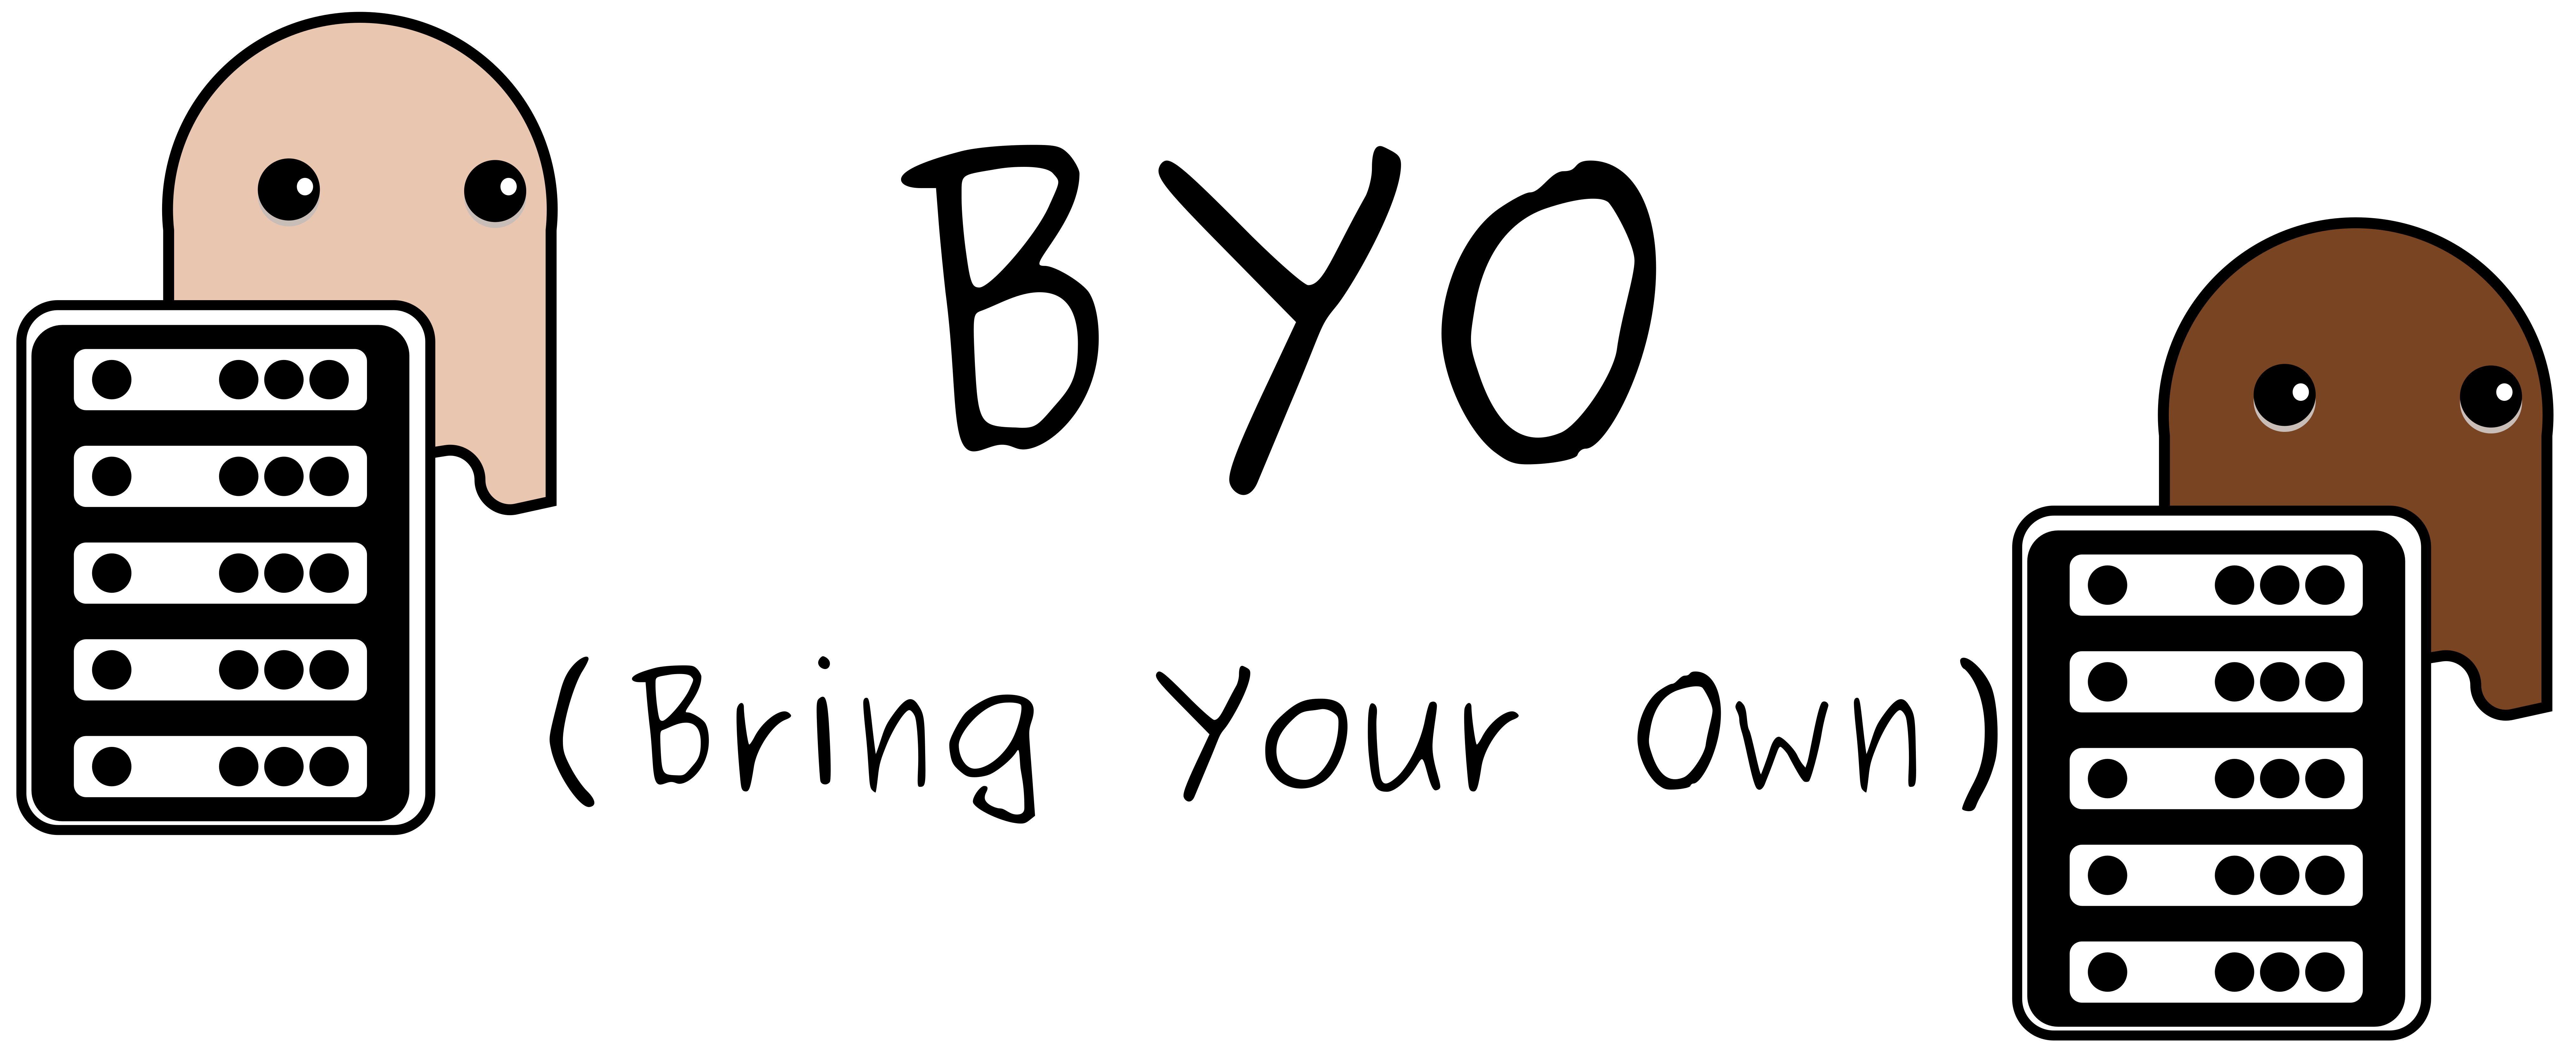
\includegraphics[width=\linewidth]{graphics/BYO.png}
	\end{figure}
\end{frame} %What to do for more control?
\begin{frame}{Advantages of using a miniHPC}
	\begin{itemize}[label={$\color{UmUBlue}\bullet$}]
		\item How many people ever get to see an HPC?
		\item It makes the hardware less abstract
		\item Real systems are busy doing actual research (85 to 95\% load on systems)
		\item Learners worried about working on a multi-million £ system
		\item Instead use low cost components that can easily be replaced - such as Raspberry Pis
		\item Resource limits more apparent
		\item More control over the environment
		\item No need to have accounts on a real HPC
		\item No need for expensive cloud hosting
		\item Own access point, so independent of university networks or the Internet
	\end{itemize}
\end{frame} %Advantages of using a miniHPC
\begin{frame}{Requirements}
	\begin{figure}
		\centering
		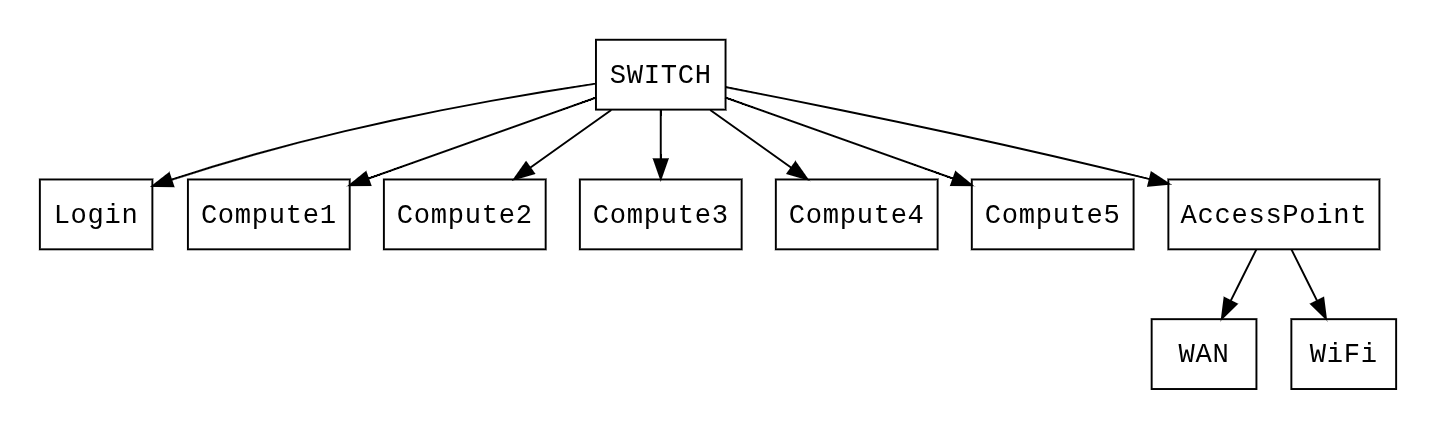
\includegraphics[width=\linewidth]{graphics/architecture.png}
	\end{figure}
	\begin{itemize}[label={$\color{UmUBlue}\bullet$}]
		\item PoE: to reduce the number of power supplies and plugs
		\item PXE: boot over Internet. No requirement for disk space on nodes
		\item One hard drive, no SD cards
		\item No requirement for Internet access
		\item Self contained with software usually available on clusters
	\end{itemize}
\end{frame} %Requirements
\begin{frame}{There are many}
	\begin{figure}
		\centering
		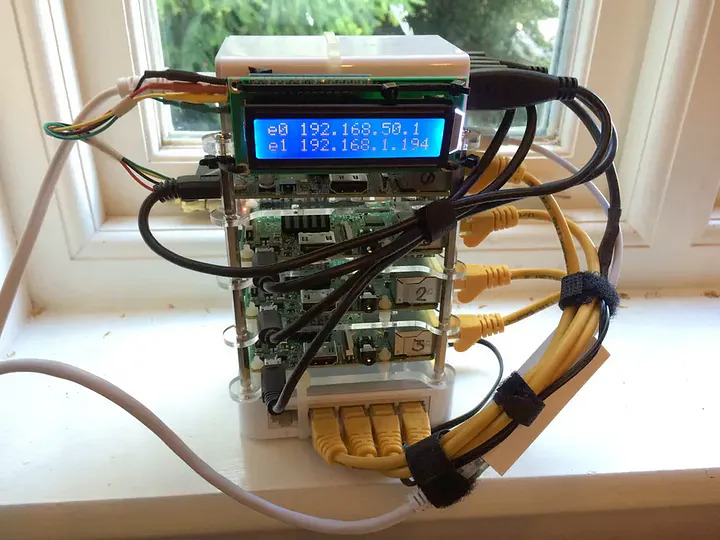
\includegraphics[width=.24\linewidth]{graphics/miniHPC1.jpg}
		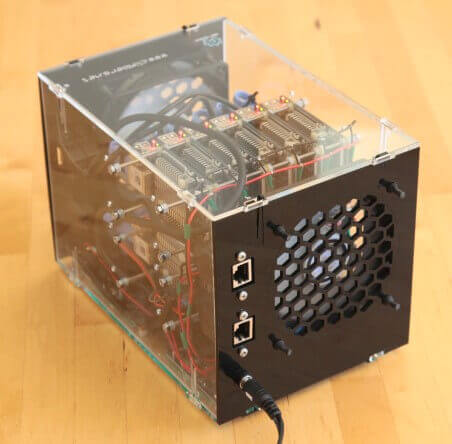
\includegraphics[width=.24\linewidth]{graphics/miniHPC2.jpg}
		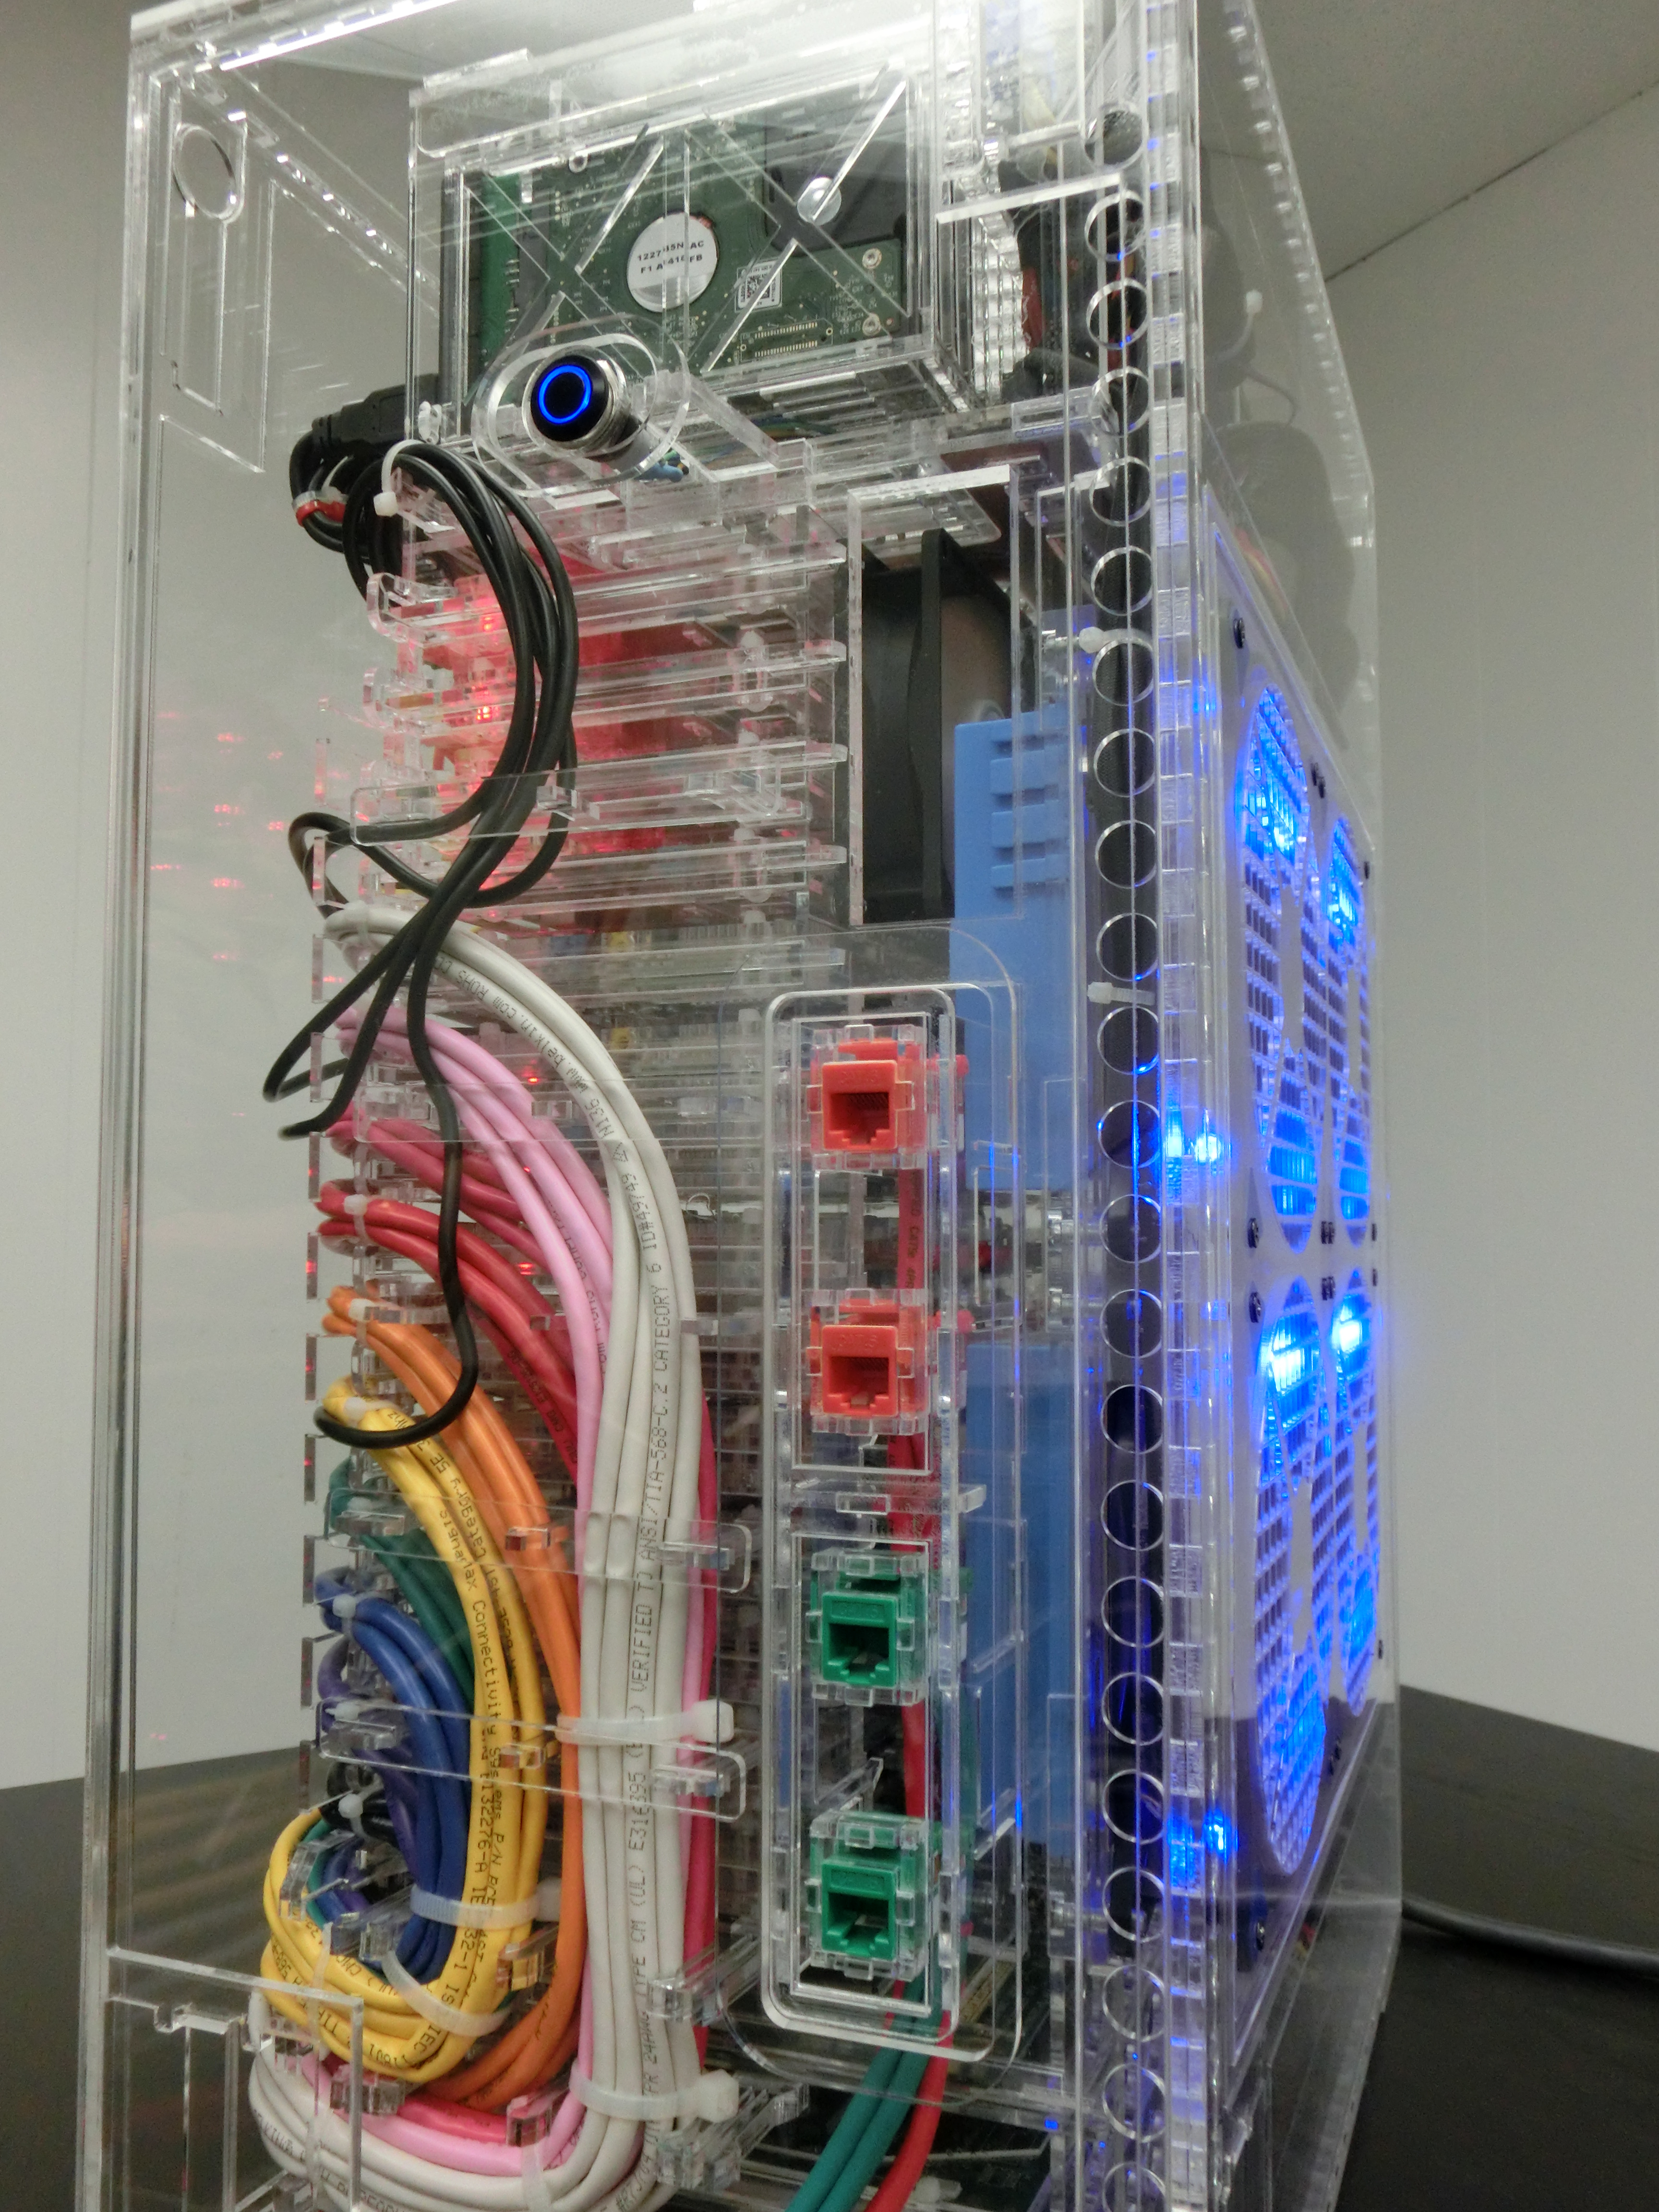
\includegraphics[width=.24\linewidth]{graphics/miniHPC3.jpg}
		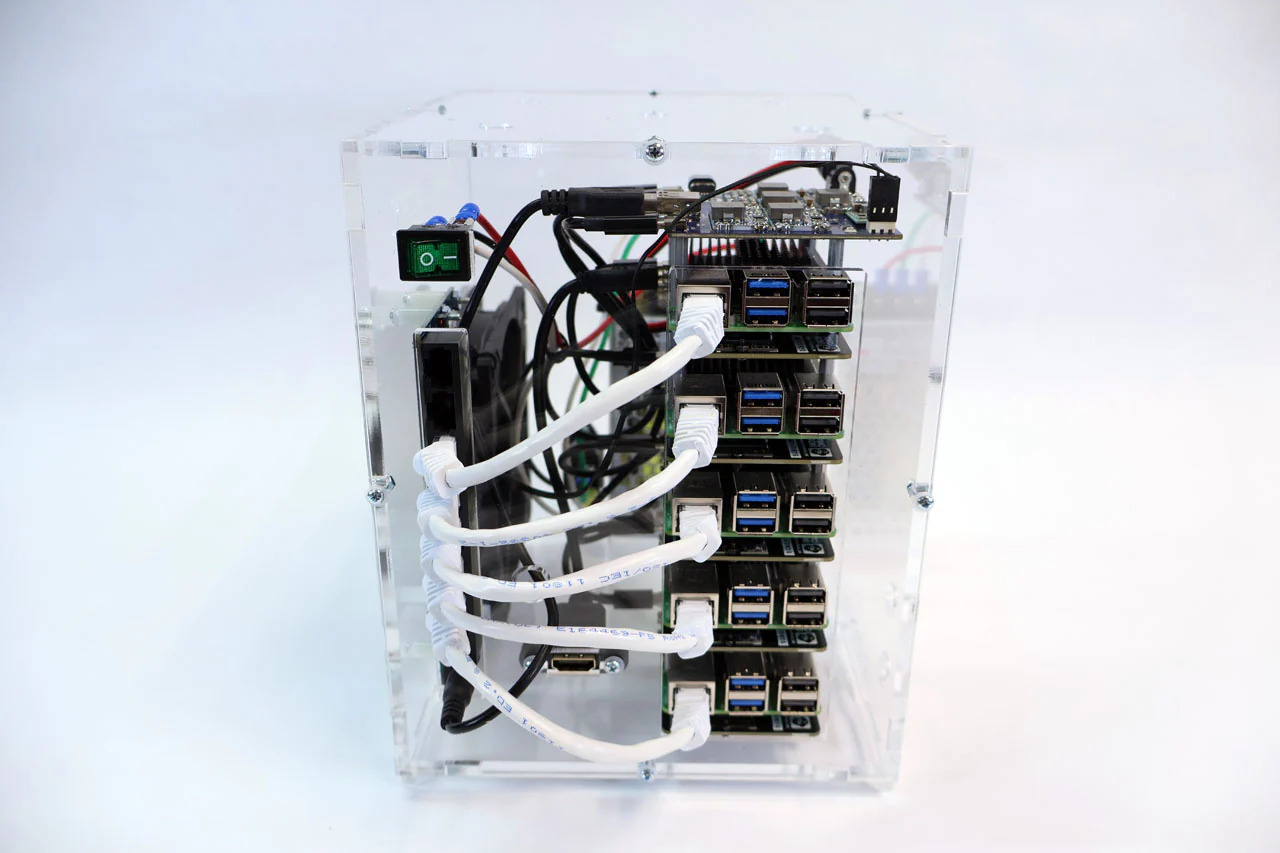
\includegraphics[width=.24\linewidth]{graphics/miniHPC4.jpg}
	\end{figure}
	
	{\tiny
		\begin{itemize}[label={$\color{UmUBlue}\bullet$}]
			\item  \url{https://aallan.medium.com/should-you-build-or-buy-a-cluster-of-single-board-computers-5931119384e8}
			\item \url{https://climbers.net/sbc/nanopi-fire3-arm-supercomputer/}
			\item \url{https://bananacluster.wordpress.com/2014/09/29/clusters-of-single-board-computers/}
			\item		\url{https://www.picocluster.com/products/pico-5m-raspberry-pi5-cluster-8gb?variant=47998253826326}

		\end{itemize}
	}
\end{frame}
 %There are many
\begin{frame}{So why yet another one?}
	\begin{columns}
		\begin{column}{0.5\linewidth}
			\begin{itemize}[label={$\color{UmUBlue}\bullet$}]
				\item Reproducibility
				\item Cost
				\item Portability
				\item Maintainability
				\item Learn about hardware
				\item Learn about software
				\item Must be useable to deliver Carpentries Intro to HPC
			\end{itemize}
		\end{column}
		\begin{column}{0.5\linewidth}
			\begin{figure}
				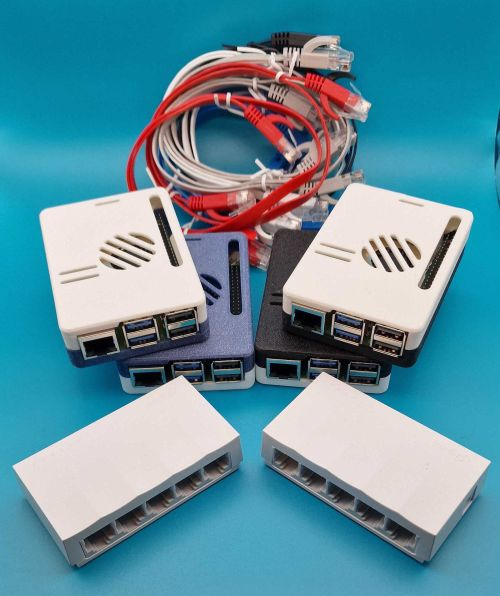
\includegraphics[width=3.5cm]{graphics/trainingkit.jpg}
			\end{figure}
		\end{column}
	\end{columns}
\end{frame}
 %So why yet another one?
\begin{frame}{Options considered}
	\begin{columns}
		\begin{column}{0.5\textwidth}
			\begin{itemize}[label={$\color{UmUBlue}\bullet$}]
				\item Several SBCs available
				\item Initially looked at RockPi 4C
				\item Circumstances led to Raspberry Pi 4
				\item Info claimed both capable of PXE
				\item PoE hats available for both
			\end{itemize}
		\end{column}
		\begin{column}{0.5\textwidth}
			\begin{figure}
				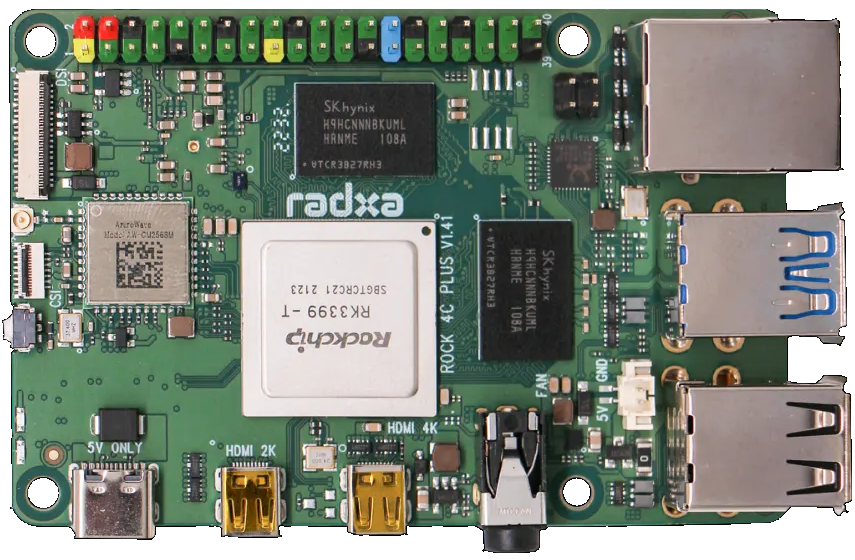
\includegraphics[width=3.5cm]{graphics/rock4c+.png}
				\caption{RockPi 4C+}
				% https://uk.rs-online.com/web/p/rock-sbc-boards/2493158
			\end{figure}
			\begin{figure}
				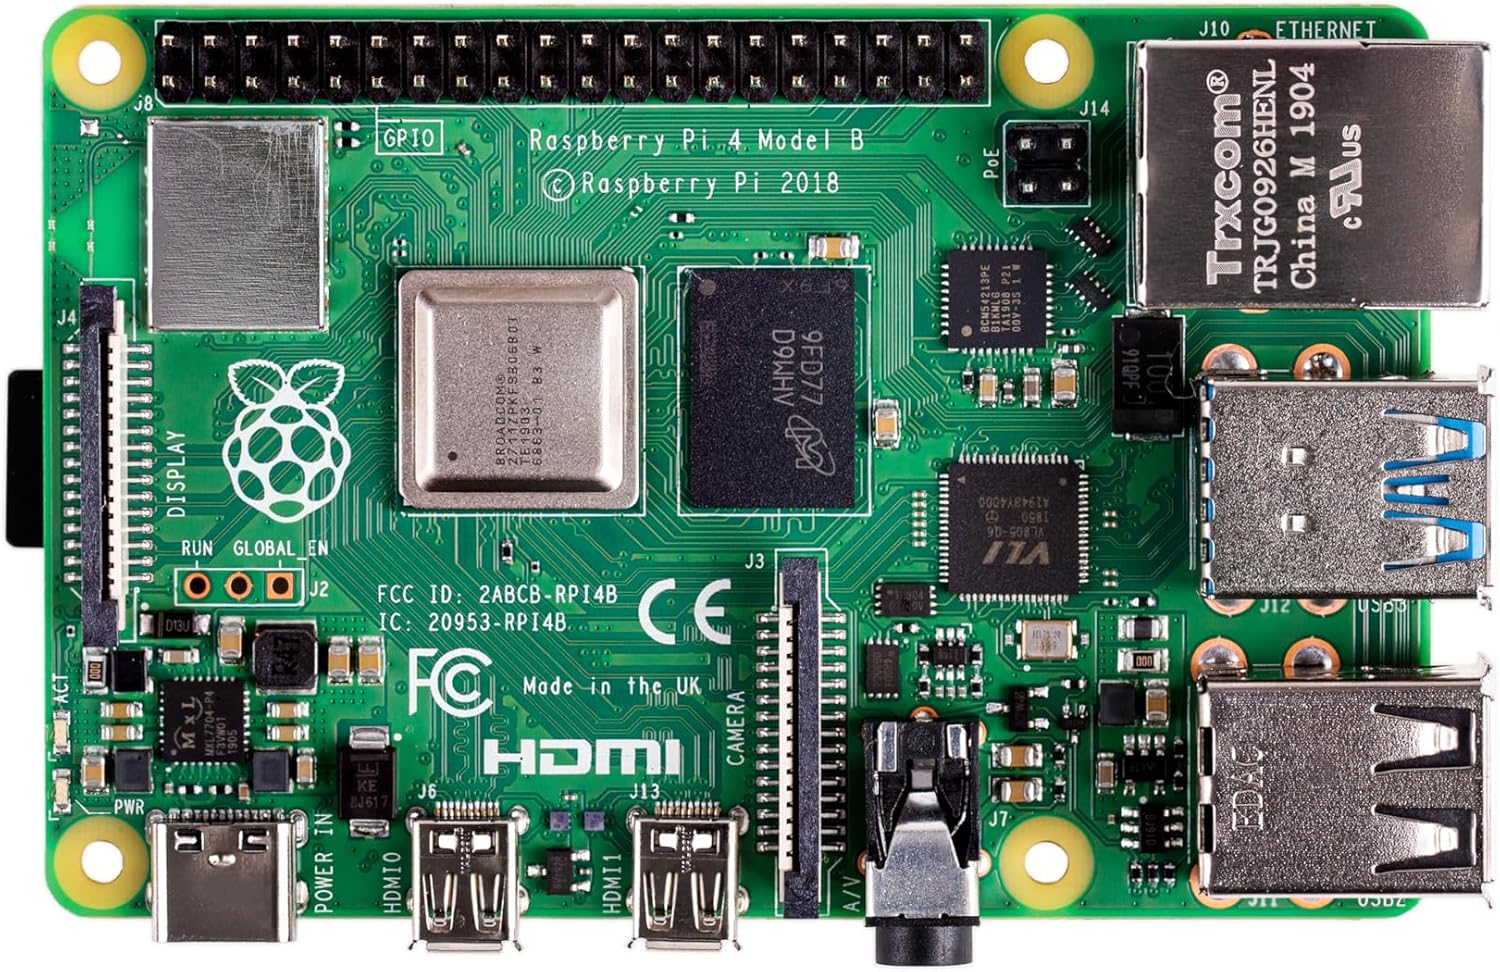
\includegraphics[width=3.5cm]{graphics/rasp4b.jpg}
				\caption{Raspberry Pi 4B}
			\end{figure}
		\end{column}
	\end{columns}
\end{frame}
 %Options considered
\begin{frame}
	\frametitle{Hardware}
	\framesubtitle{Six node specification}
	\begin{itemize}
		\item 1 x Login node
		\item 5 x Compute nodes
		\item 1 x Access point
		\item 1.8GHz Broadcom BC2711, Quad core Cortex-A72 (ARM v8 64 bit SoC)
		\item 4GB RAM
		\
	\end{itemize}
\end{frame}
 %Hardware: Six node specification
\begin{frame}
	\frametitle{Hardware}
	\framesubtitle{Shopping list and costs}
	\begin{table}[]
		\begin{tabular}{l|rcr}
			\hline
			\textbf{Item} & \textbf{Cost} & \textbf{Qty} & \textbf{Total} \\ \hline
			\textbf{Raspberry Pi 4B} & £34.00 & 7 & £204.00\\ 
			\textbf{PoE Hat} & £20.00 & 7 & £140.00\\ 
			\textbf{10 port switch with 8 x PoE} & £190.00 & 1 & £190.00\\
			\textbf{Patch cable - pack of 8} & £10.00 & 1 & £10.00\\
			\textbf{USB to SATA Adapter} & £9.00 & 1 & £9.00\\
			\textbf{120GB SATA SSD} & £10.00 & 1 & £10.00\\
			\textbf{80mm 5V USB fans - pack of 2} & £10.00 & 1 & £10.00\\
			\textbf{10" GeeekPi Rack} & £110.00 & 1 & £110.00\\
			
			\hline
			\textbf{Total} & & & £683.00\\
			\hline
		\end{tabular}
		\caption{Raspberry Pi 4B option}
		\label{tab:1}
	\end{table}
\end{frame}

 %Hardware: Shopping list and costs
\begin{frame}
	\frametitle{Hardware}
	\framesubtitle{The Evolution of a miniHPC}

	\begin{figure}
		\centering
		\begin{subfigure}[b]{0.24\textwidth}
			\centering
			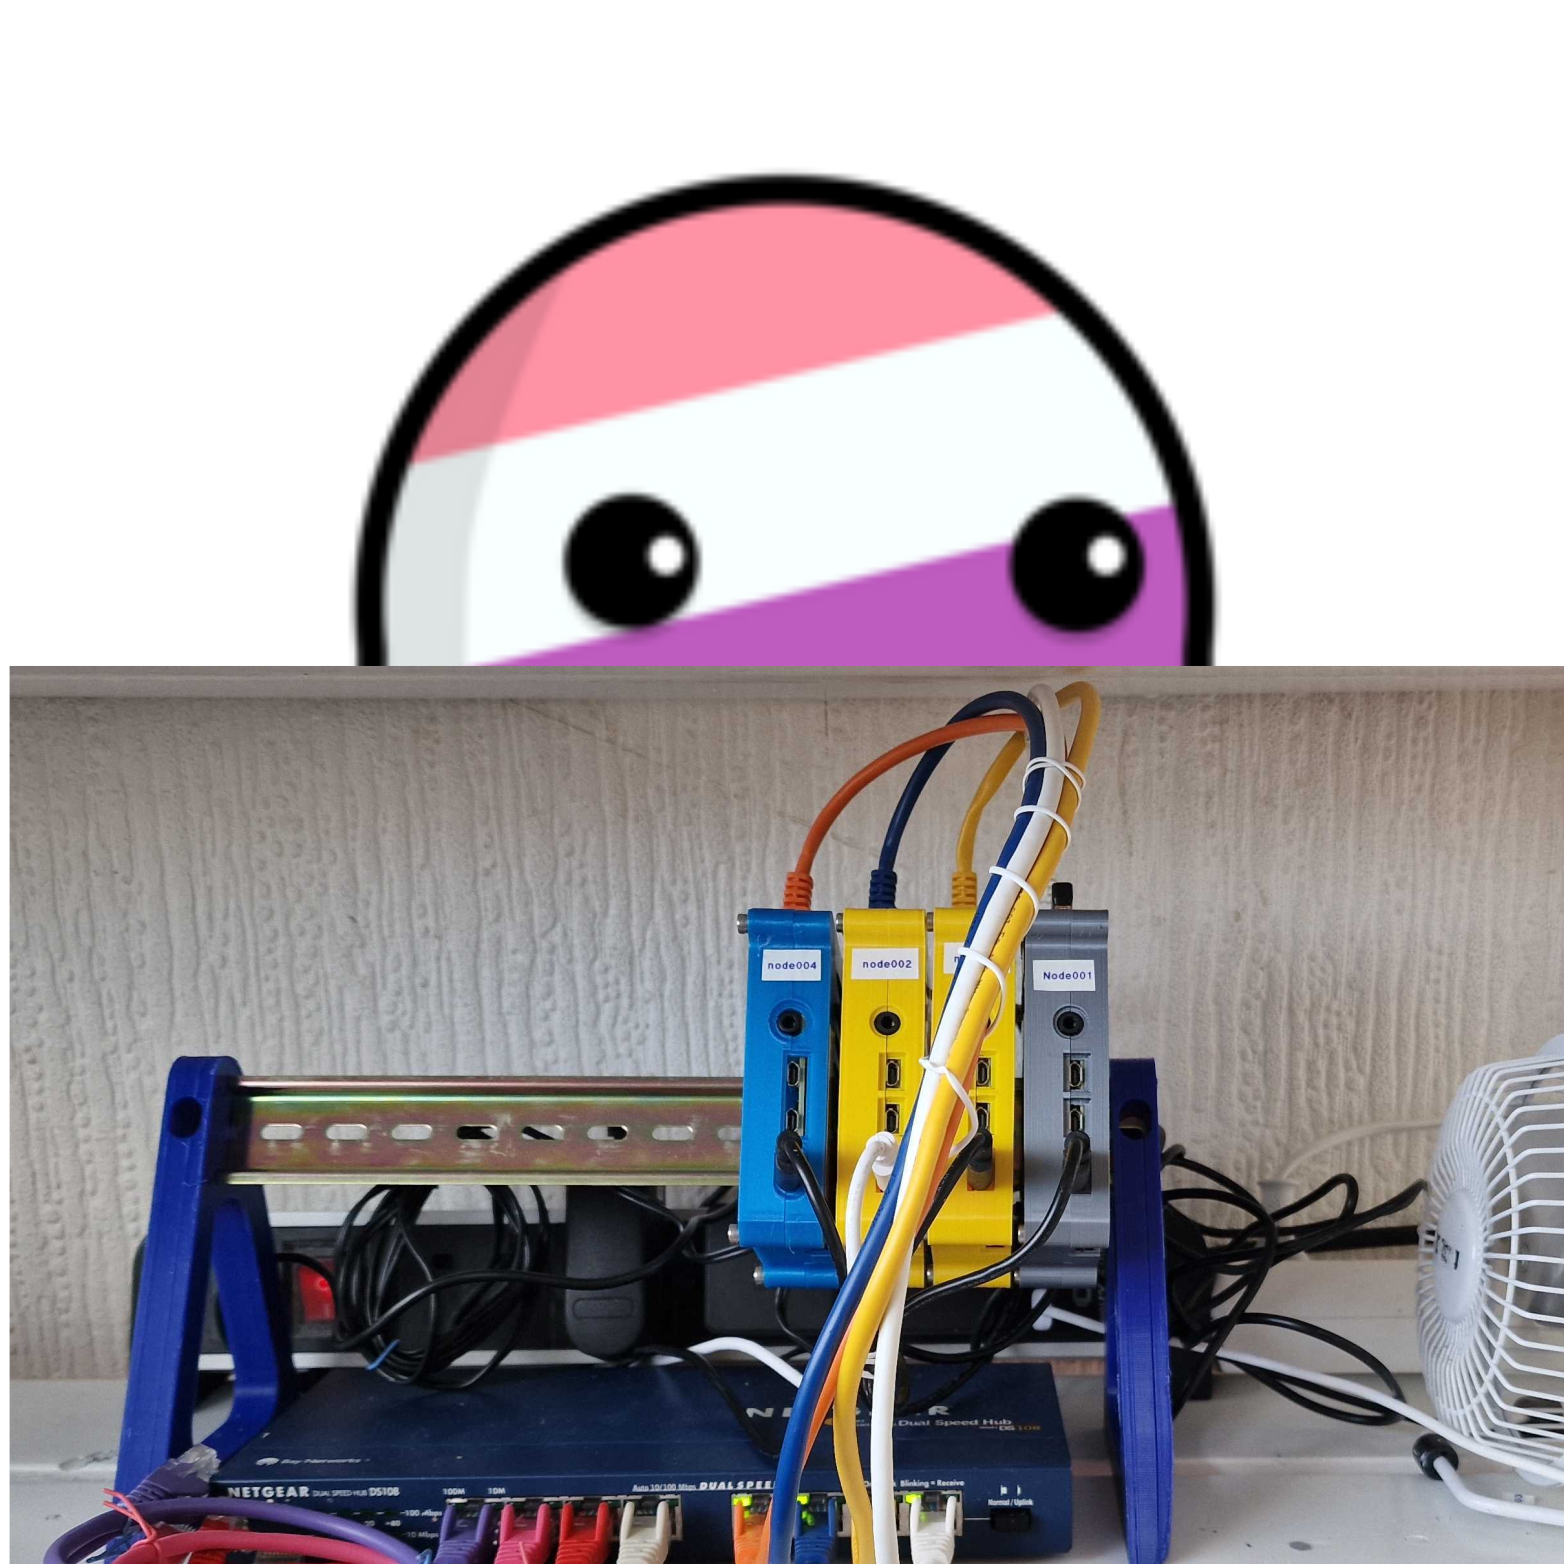
\includegraphics[width=\textwidth]{graphics/barba_with_miniHPC.png}
			\caption{Prototype 1}
			\label{fig:2.a}
		\end{subfigure}
		\hfill
		\begin{subfigure}[b]{0.24\textwidth}
			\centering
			\includegraphics[width=\textwidth]{graphics/mini-HPC-proto2.png}
			\caption{Prototype 2}
			\label{fig:2.b}
		\end{subfigure}
		\hfill
		\begin{subfigure}[b]{0.24\textwidth}
			\centering
			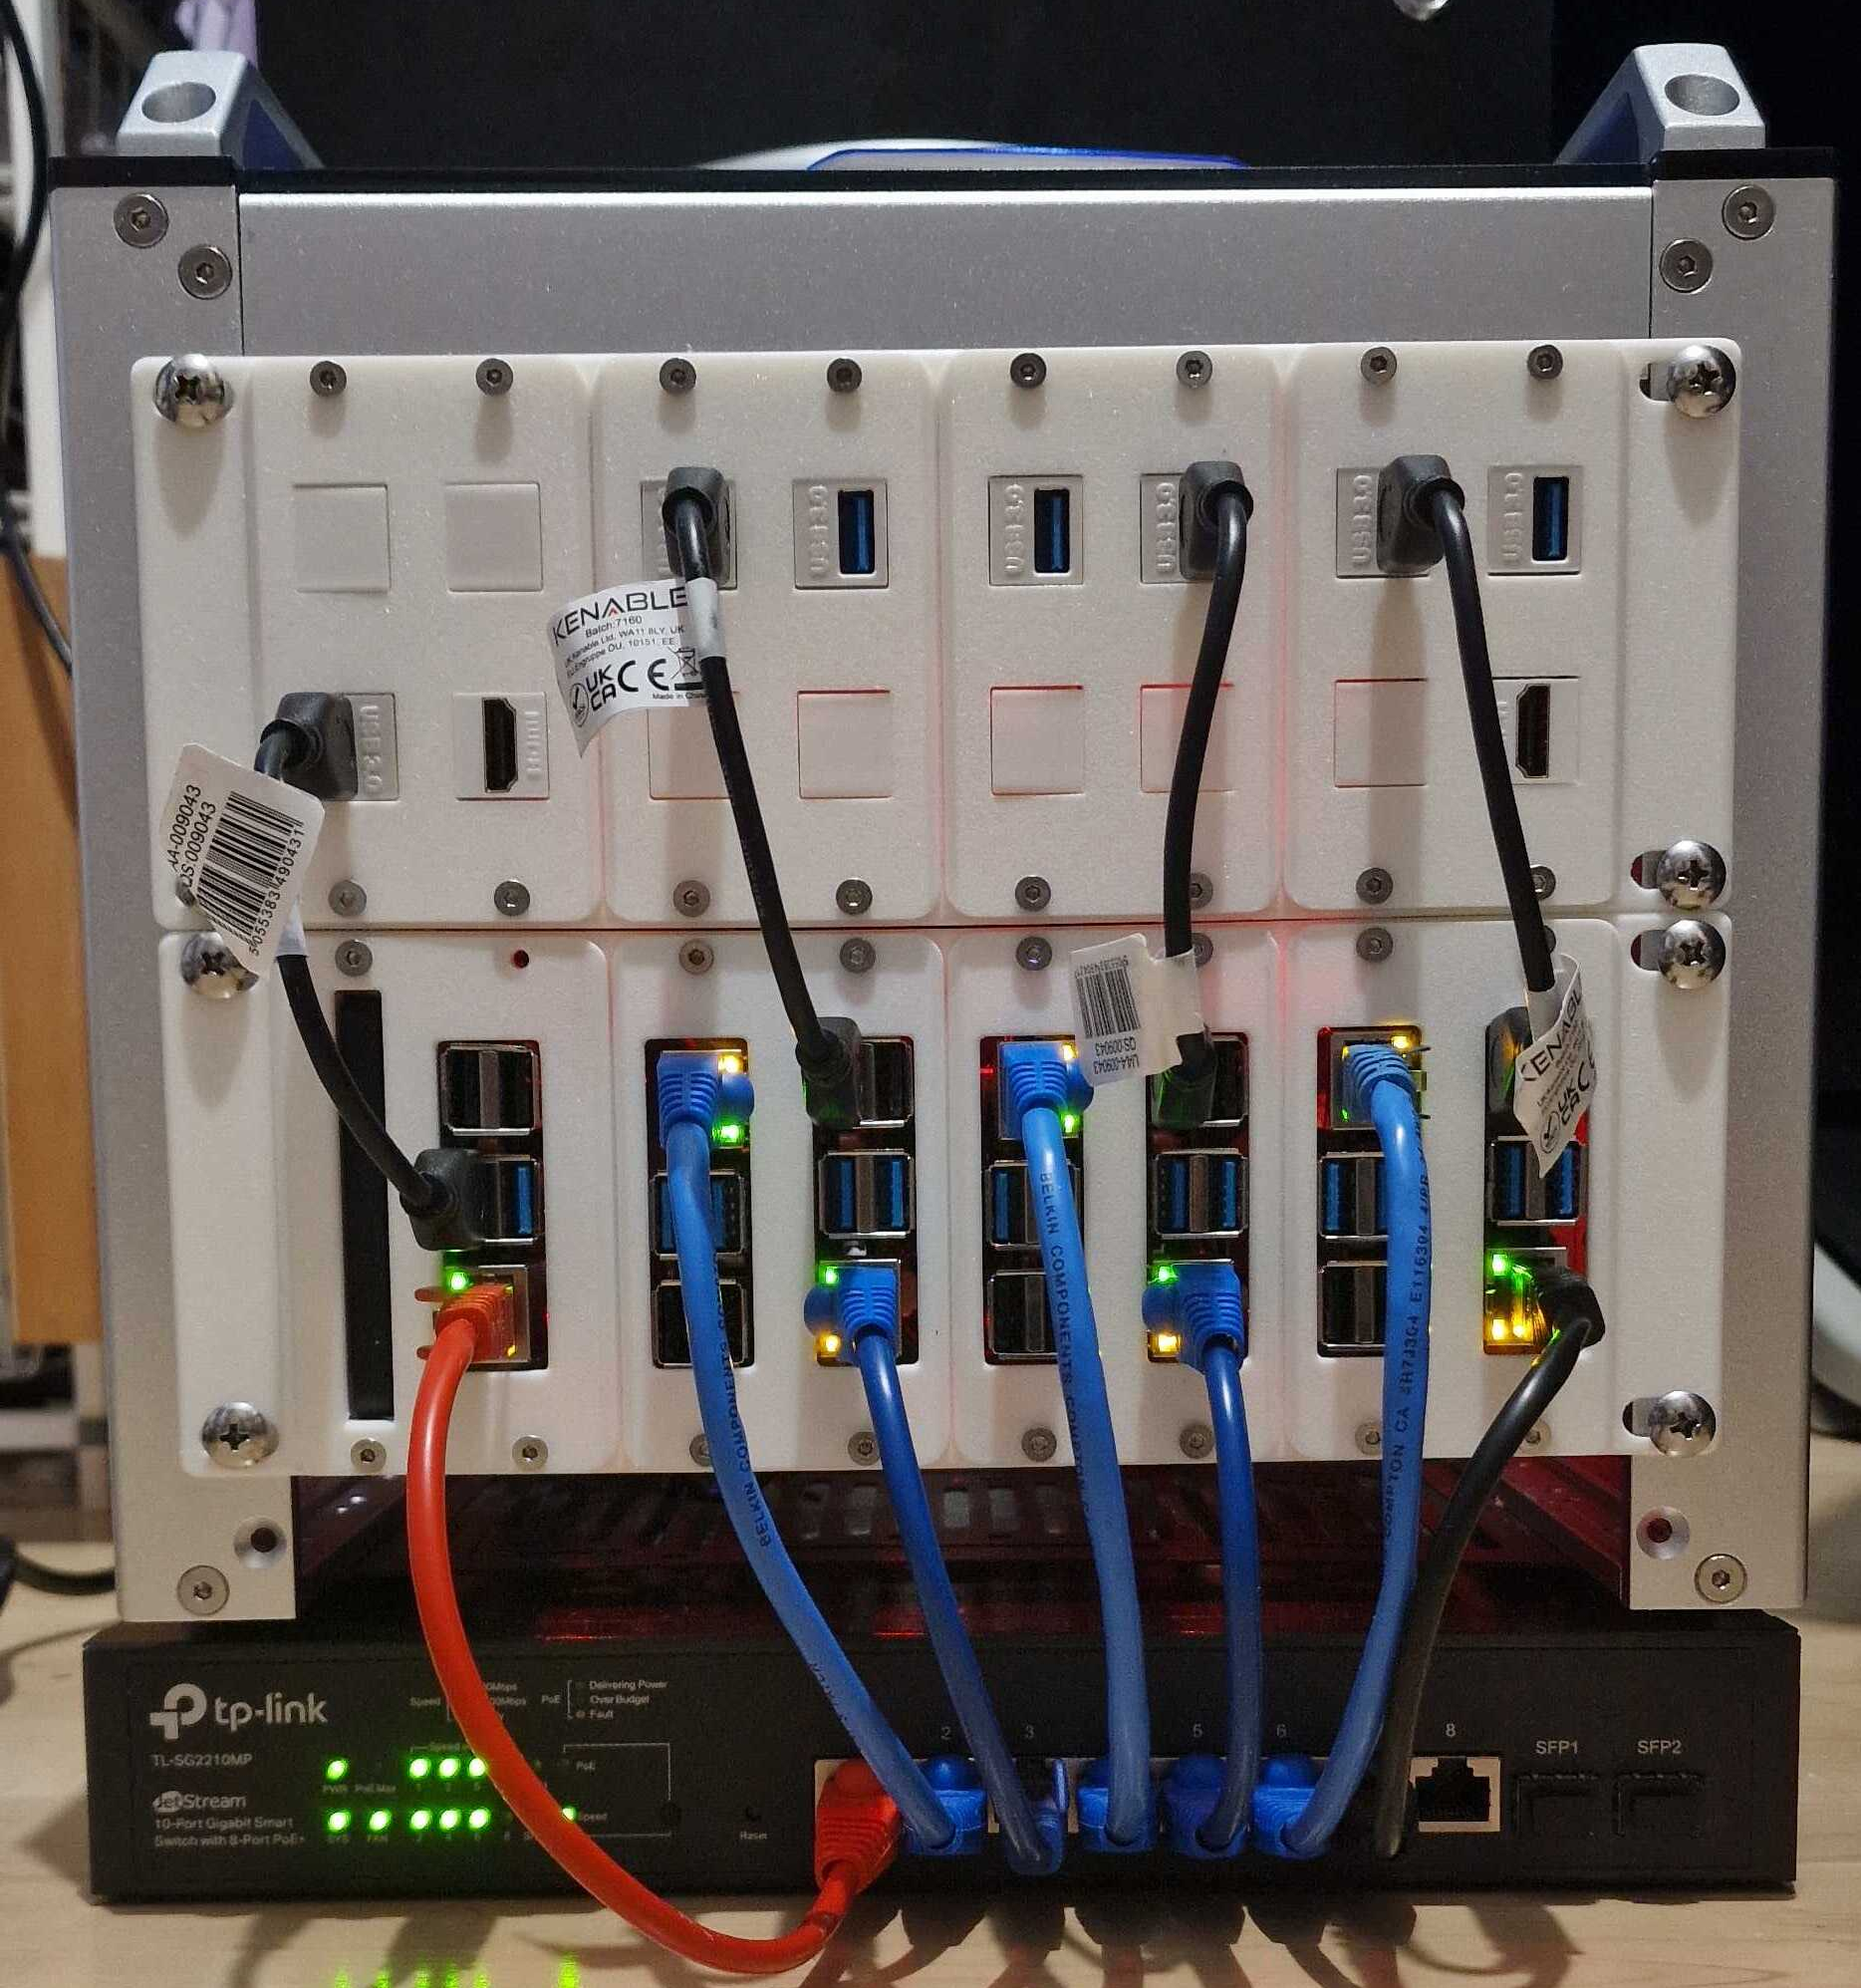
\includegraphics[width=\textwidth]{graphics/mini-HPC-proto3.png}
			\caption{Prototype 3 front}
			\label{fig:2.c}
		\end{subfigure}
		\hfill
		\begin{subfigure}[b]{0.24\textwidth}
			\centering
			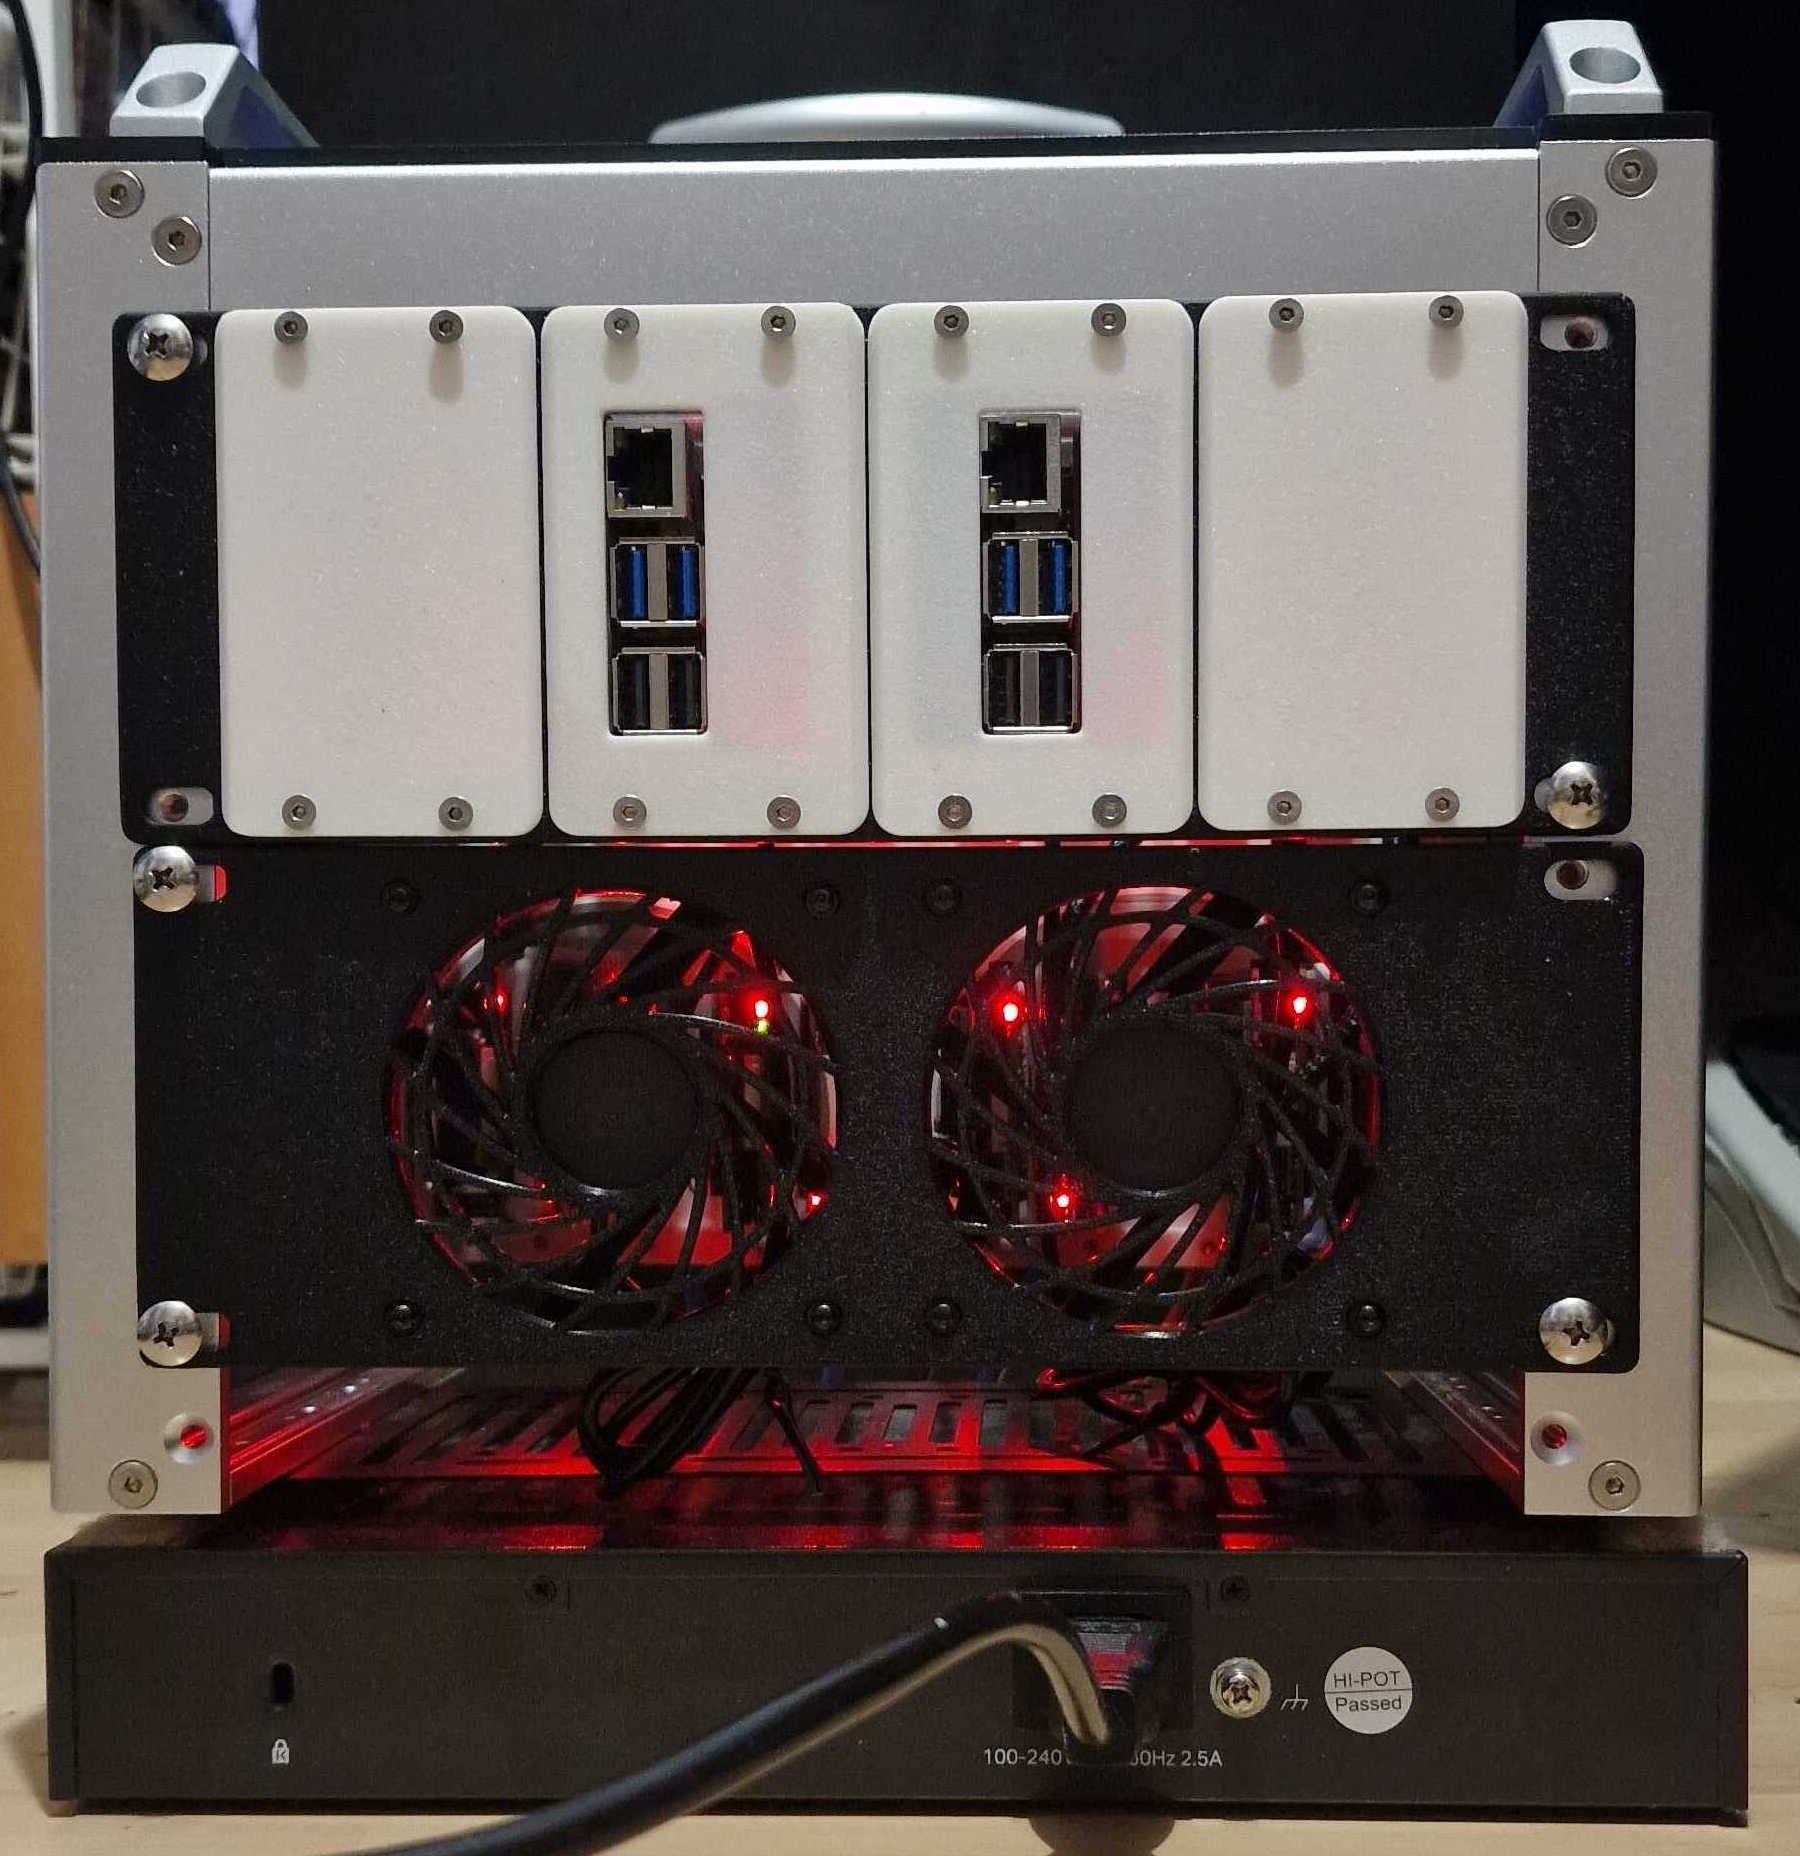
\includegraphics[width=\textwidth]{graphics/mini-HPC-proto3_back.png}
			\caption{Prototype 3 back}
			\label{fig:2.d}
		\end{subfigure}

		\label{fig:2}
	\end{figure}
	
\end{frame}
 %Hardware: The Evolution of a miniHPC

\begin{frame}
	\frametitle{Hardware}
	\framesubtitle{Almost (but not quite) finally}
	\begin{figure}
		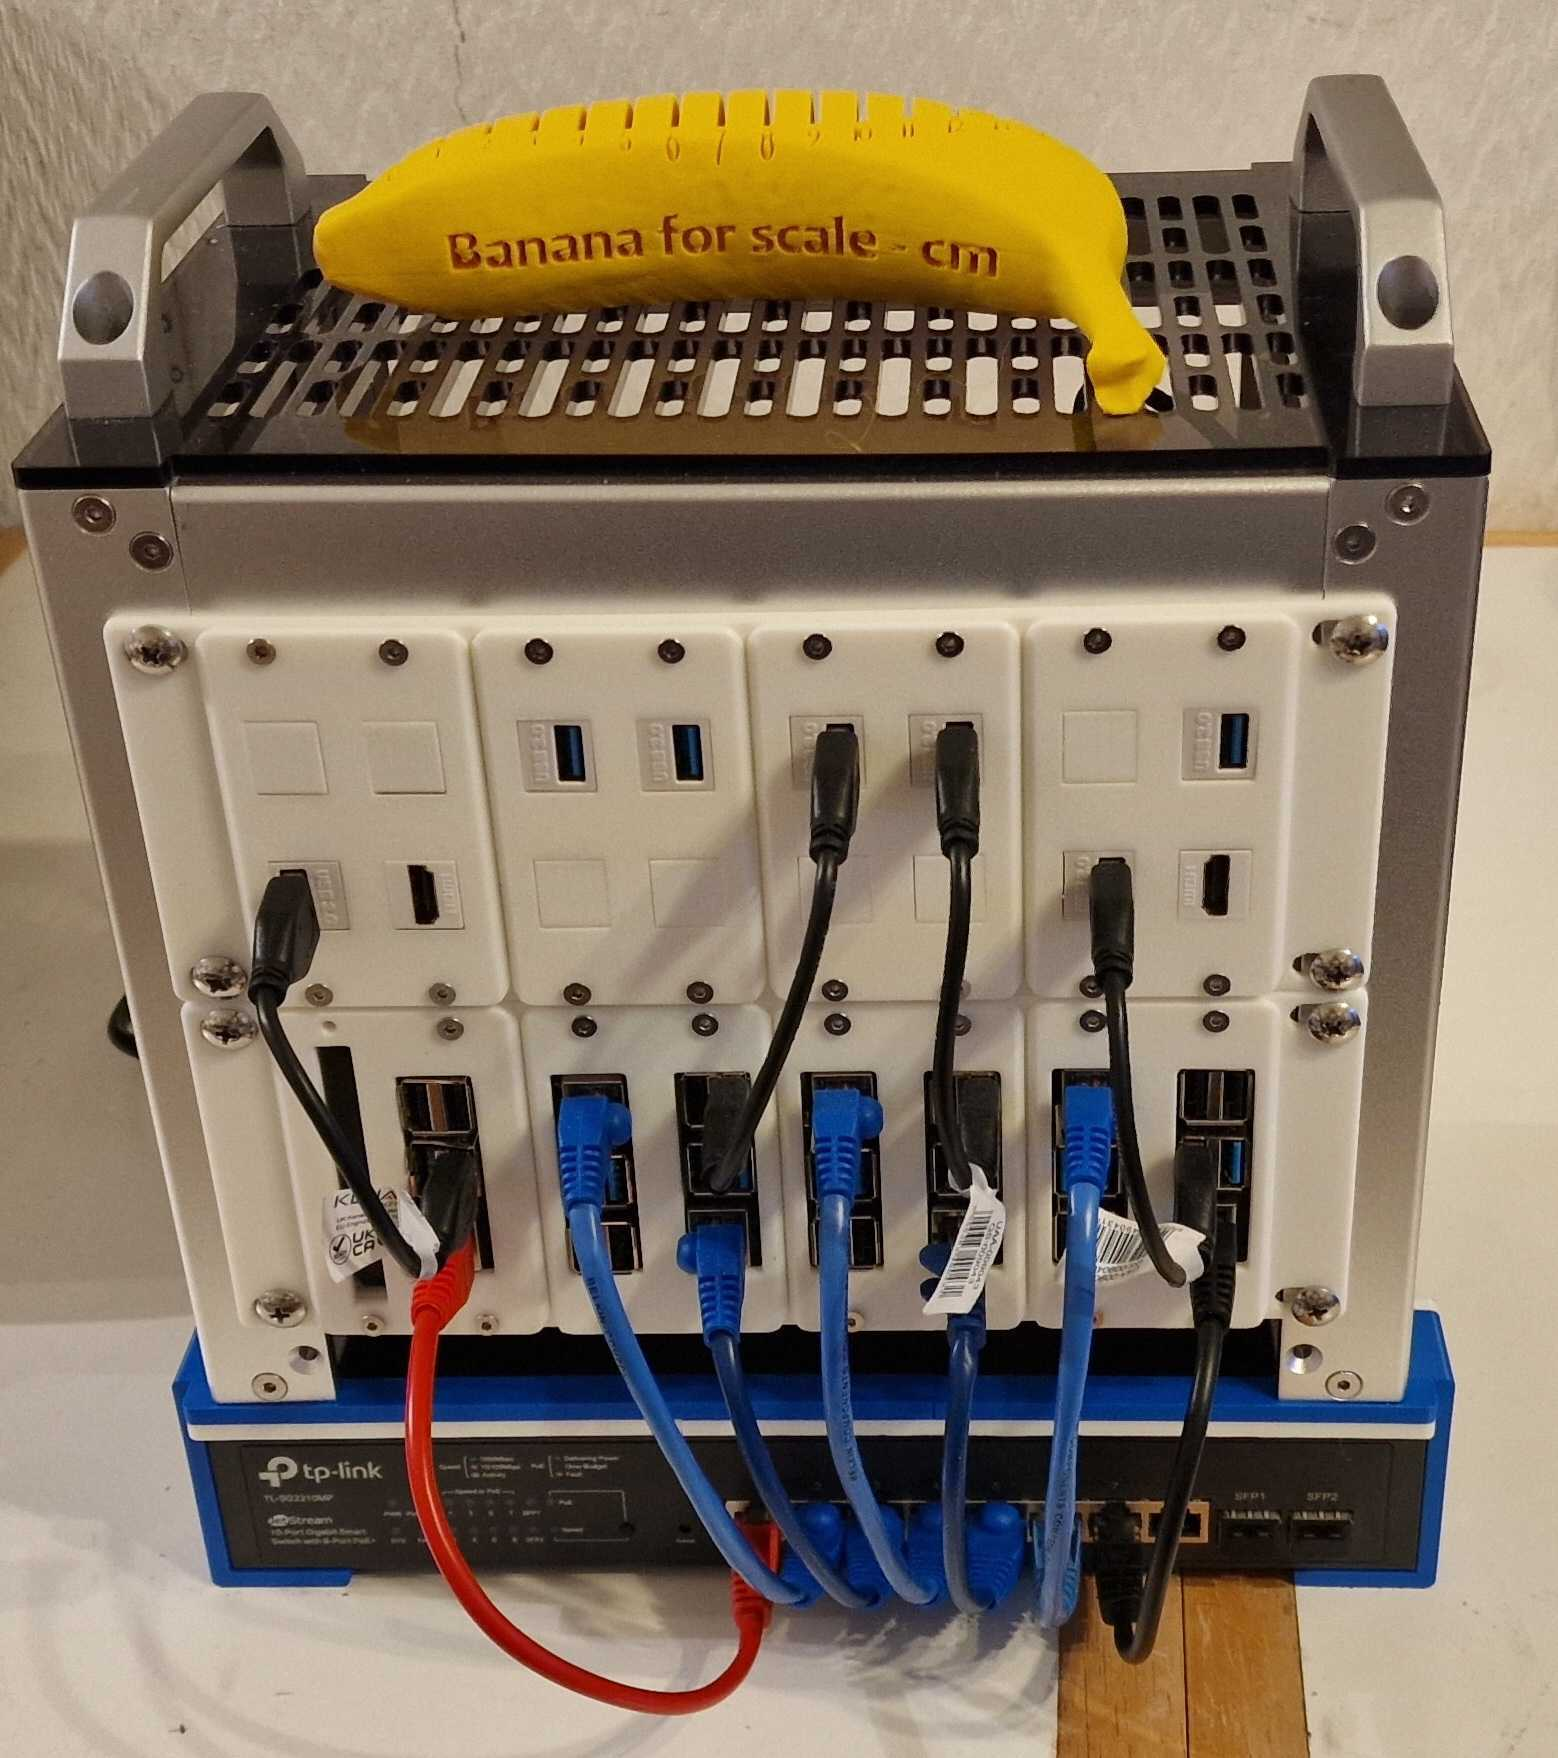
\includegraphics[height=0.60\textheight]{graphics/banana_for_scale.jpg}
		\caption{{\large\bf{Now}} with a bracket that fixes the switch to the cabinet, and a banana for scale. \linebreak
			{\tiny(It still needs Internet access)}}
	\end{figure}
\end{frame} %Hardware: Almost (but not quite) finally
\begin{frame}
	\frametitle{Software}
	\framesubtitle{Standard HPC Software}
	
	\begin{columns}[T]
		\begin{column}[c]{.5\textwidth}
			\begin{itemize}[label={$\color{UmUBlue}\bullet$}]
				\item Slurm scheduler
				\item Shared NFS mounts
				\item lmod
				\item munge
				\item EESSI for software installations
			\end{itemize}
		\end{column}
		\begin{column}[c]{.5\textwidth}
			\centering
			
\includegraphics[width=.8\textwidth]{graphics/logos.png}
		\end{column}
	\end{columns}
\end{frame}
 %Standard HPC Software
\begin{frame}
	\frametitle{The CarpentriesOffline Solution}
	\framesubtitle{Making it easier for non-specialists}
	
	\begin{columns}
		\begin{column}[c]{.60\linewidth}
			\begin{itemize}[label={$\color{UmUBlue}\bullet$}]
				\item Downloadable image for booting RPi​
				\item No specialised HPC knowledge required to set up
				\item Community maintained (The Carpentries way)
				\item HPC Lesson material adapted for miniHPC
				\item Expandable with regards to hardware and software
				\item Also suitable for HPC hardware and config training
			\end{itemize}
		\end{column}
				
		\begin{column}[c]{.35\linewidth}
			\begin{figure}
				\includegraphics[width=.8\textwidth]{graphics/training_kit.png}
			\end{figure}
		\end{column}
	\end{columns}
\end{frame} %Making it easier for non-specialists
\begin{frame}
	\frametitle{}
	\centering\LARGE Thank You For Listening \\
	\centering\LARGE Any Questions?
	\begin{columns}[b]
		\begin{column}[b]{.35\linewidth}
			\begin{figure}
				
\includegraphics[width=.5\textwidth]{graphics/www.jannetta.com.png}
				\caption{www.jannetta.com}
			\end{figure}
		\end{column}
		\begin{column}[b]{.35\linewidth}
			\begin{figure}
				
\includegraphics[width=.5\textwidth]{graphics/carpentriesoffline.org.png}
				\caption{carpentriesoffline.org}
			\end{figure}
		\end{column}
	\end{columns}
\end{frame}
 %Thank you

%\begin{frame}{Raspberry Pi 5}
%	\begin{columns}
%		\begin{column}{0.5\textwidth}
%			\begin{itemize}[label={$\color{UmUBlue}\bullet$}]
%				\item  Funding from SSI for 8 RPi5
%				\
%			\end{itemize}
%		\end{column}
%		\begin{column}{0.5\textwidth}
%			\begin{figure}
%				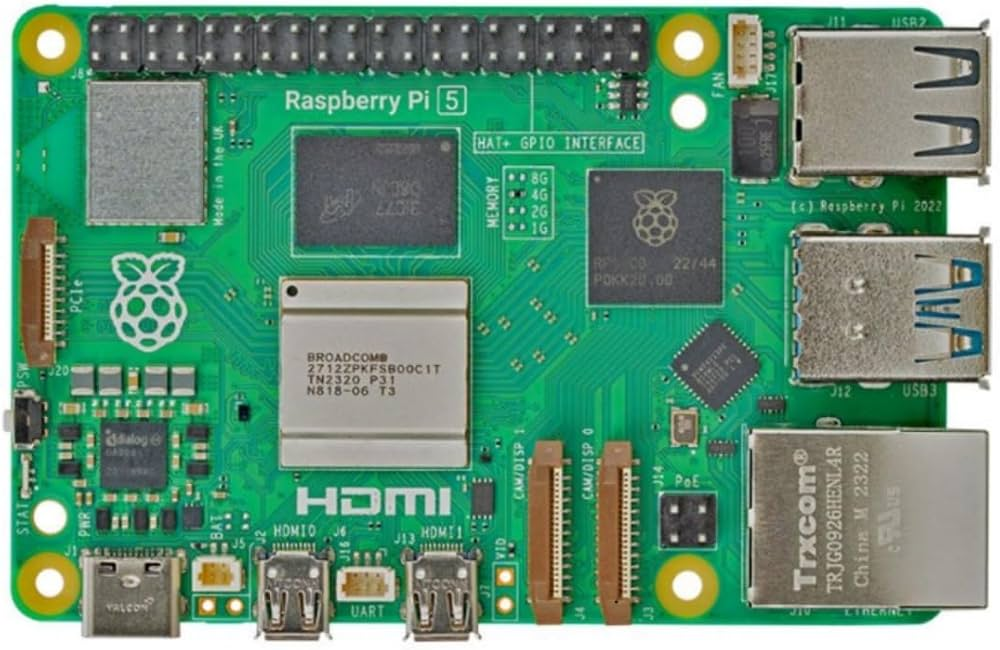
\includegraphics[width=3.5cm]{graphics/rasp5.jpg}
%				\caption{Raspberry Pi 5}
%			\end{figure}
%		\end{column}
%	\end{columns}
%\end{frame}

\end{document}